%\documentclass[12pt]{article}
% Kalman Filtering forumulation
%\usepackage{amsmath}
%\usepackage{verbatim}
%\usepackage{fixltx2e}

%\def\dfdx#1#2{\frac{\partial {#1}}{\partial {#2}}}
%\begin{document}
%\newpage
\chapter{Modelling}
This chapter discusses two modelling approaches used in the Kalman filter.
% Multi body system 
In the first approach, the robot is modelled as multi body dynamic system in which the motion of the robot is caused by application of torques at the respective joints.
% sensor fusion
In the second approach a simplified model of a inertial navigation system is considered to estimate the motion of the robot.
\section{Multi body system}
Humanoid robots consists of group of rigid bodies that are joined together to resemble the human skeletal structure. As human beings are driven by the muscular system, humanoids are driven by electric, hydraulic or pneumatic actuators, which apply torques at the joints of the robot. The dynamics of robots describes how the robots moves in response to the actuator forces or torques. The dynamics of the robot is defined by the  equations of motion of the rigid body system. In general there are several approaches in deriving equations of motion of rigid body dynamic system. One such approach is by deriving Lagrange equation. Lagrangian analysis relies on the energy properties of the mechanical system to derive the equations of motion. The \emph{Lagrangian, L,} is defined as the difference between kinetic and potential energy of the system. $$ L(q,\dot{q}) = T(q,\dot{q}) - V(q)$$ \emph{q} represents the vector of joint angles \emph{T} and \emph{V} represents the kinetic and potential energies of the system. \emph{q} is called the generalized coordinates of the system as the specification of joint angles uniquely determines position of all the rigid bodies.

The equations of motion for a rigid body system with generalized coordinates $q \in \Re^m $ is given by,
\begin{equation}
\frac{d}{dt} \dfdx{L}{\dot{q}}-\dfdx{L}{q_i} = \Gamma_i   i = 1,...,m
\end{equation}
$\Gamma_i$ is the external force acting on the ith generalized coordinate.
\begin{figure}
\begin{center}
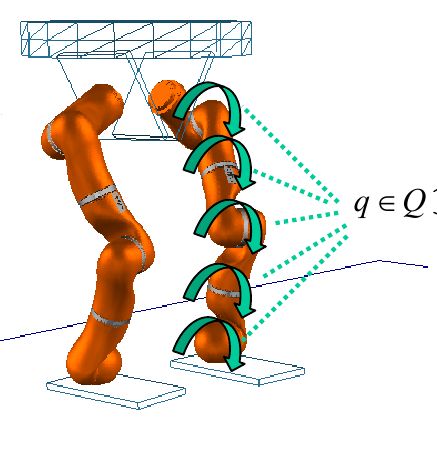
\includegraphics[scale=0.75]{Bilder/model_biped.png}
\caption{Simplified lower body model of biped}
\label{fig:biped_simplelow}
\end{center}
\end{figure}
The general formulation of equation of motion of biped shown in Figure \ref{fig:biped_simplelow} with configuration space \emph{Q} is
\begin{equation}
M(q)\ddot{q}+C(q,\dot{q})+g(q) = \tau
\end{equation}
\emph{M(q)} is the generalized inertia matrix, $C(q,\dot{q})$ is the matrix representing Coriolis and centrifugal forces, \emph{g(q)} is the gravity vector acting on the system and $\tau$ is the actuator torque applied to the joints.

\emph{Toro} is modelled as floating base dynamic model.
\begin{equation}
	\label{eq:motion}
	\begin{split}
	\ddot{q} = M(q)^{-1}(&-C(q,\dot{q})\dot{q} - g(q) + (J_{bl}^{b})^{T}F_{l}^{b} +(J_{br}^{b})^{T}F_{r}^{b} + \tau) \\
	\text{where,}\\
	q_{base} &= (p_{f}^{T},\theta_{f}^{T})^{T} \in \Re^{6} \\
	q_{j} &= (q_{1},q_{2},\ldots , q_{25})^{T} \in \Re^{25}\\
	q &= (q_{f}^{T}, q_{j}^{T})^{T} \in \Re^{31}\\
	\end{split}
\end{equation}
\emph{q} is the generalized coordinates. The coordinates of the floating base $q_{f}$ are defined with reference to spatial frame, whereas $q_{j}$ are defined with reference to body frame. $q_{f} = (p_{f}^{T},\theta_{f}^{T})^{T}$, where $p_{f}=(x,y,z)^{T}$ is a vector representing  the position of origin of floating base in spatial frame and $\theta_{f}=(\theta_{x},\theta_{y},\theta_{z})^{T}$ is a vector of Euler angles that describes the rotation of base frame with respect to spatial frame.$q_{j} \in \Re^{25}$ is the vector of joint angles. $\dot{q} =  (\hat{V}_{f}^{b},\dot{q_{j}})^{T} \in \Re^{31}$ is the vector of generalized velocities. $\hat{V}_{f}^{b} = (v_f^b,\omega_f^b)^T \in \Re^{6}$ is the body twist. $\dot{q}_{j} \in \Re^{25}$ is the vector of joint velocities. $\ddot{q}\in \Re^{31}$ is the vector of generalized accelerations. $M(q)\in \Re^{31 \times 31}$ is the inertia matrix, $C(q,\dot{q})\in \Re^{31 \times 31}$ is the matrix accounting for centrifugal and Coriolis forces. $g(q) \in \Re^{31}$ is the gravity vector. $\tau \in \Re^{31}$ is the vector of actuating torques acting on $q_{j}$, where the first six components are zero because those degrees of freedom corresponding to $q_{f}$ are not actuated.$(J_{br}^{fb})^{T},(J_{bl}^{fb})^{T} \in \Re^{31 \times 6}$ are the Jacobian matrices transforming the wrenches $F_{r}^{fb},F_{l}^{fb} \in \Re^{6}$ applied in the right and left foot to joint torques.
\paragraph{State Space representation:}
General state space representation of a non linear system
\begin{equation}
\label{eq:dyn_nl}
	\begin{split}
	\dot{x} = f(x,u)\\
	y = h(x,u)
	\end{split}
\end{equation}
where, $x \in \Re^{n}$ is the vector representing the states of the system. $u \in \Re^{p}$ is the vector of inputs acting on the system. $y \in \Re^{m}$ is the vector of outputs of the system.\\
State space representation of \emph{Toro}
\begin{equation}
\label{eq:toro}
	\begin{split}
	\dot{x} = &
	\begin{pmatrix}
	R_{sb}\dot{p}_f\\
	T(\theta_{f})^{-1}R_{sb}\omega_f^b \\
	\dot{q}_{j}\\
	M(q)^{-1}(-C(q,\dot{q})\dot{q} -g(q) + (J_{bl}^{b})^{T}F_{l}^{b} +(J_{br}^{b})^{T}F_{r}^{b} + \tau)	
	\end{pmatrix}
	\\&	y = 
	\begin{pmatrix}
	q_{j} \\ \dot{q}_{j} \\ \ddot{p}_{f}^b \\ \omega_{f}^{b}\\ p_{c}^{b}\\ \hat{V}_{c}^{b}
	\end{pmatrix}
	\\ \text{where, }\\ x &= (q^{T},\dot{q}^{T})^{T} \in \Re^{62}\\
	%\begin{comment}
	%	T_{A}(\theta_{f}) &=
	%\begin{pmatrix}
	%\textbf{I} &\textbf{0} \\
	%\textbf{0} &T(\theta_{f})
	%\end{pmatrix} 
	%\end{comment}
	\\T(\theta_{f}) &=
	\begin{pmatrix}
	1 &0 &\sin(\theta_{y})\\
	0 &\cos(\theta_{x}) &-\sin(\theta_{x})\cos(\theta_{y})\\
	0 &\sin(\theta_{x}) &\cos(\theta_{x})\cos(\theta_{y})\\
	\end{pmatrix}	\\
	\ddot{p}_{f}^{b} &= \ddot{q}(1,2,3)^{T} + R_{sb}^{T} 
	\begin{pmatrix}
	0 \\ 0 \\ 9.81
	\end{pmatrix}\\
	%\dot{\theta}_{f}^{b} &= R_{sb}^{T}T(\theta_{f})^{-1}R_{sb}\omega_{f}^{b}\\
	p_{c}^{b} &= (p_{a,r}^{b}, p_{b,r}^{b}, p_{a,l}^{b}, p_{b,l}^{b} )^{T} \\
	 \text{ i.e } &p_{a,r}^{b} = H_{sr}^{-1} p_{a,r}^{s},p_{b,r}^{b} = H_{sr}^{-1} p_{b,r}^{s},p_{a,l}^{b} = H_{sl}^{-1} p_{a,l}^{s},p_{b,l}^{b} = H_{sb}^{-1} p_{b,l}^{s}  \\
	\hat{V}_{c}^{b} &= (\hat{V}_{r}^{b},\hat{V}_{l}^{b})^{T} \text{ i.e } \hat{V}_{r}^{b} = J_{r}\dot{q} \text{ and } \hat{V}_{l}^{b} = J_{l}\dot{q}
	\end{split}
	\end{equation}
\begin{itemize}
\item $T(\theta_{f})$ is the matrix that transforms the angular velocity $\omega_{f}^{s}$ to the time derivative of Euler angles $\dot{\theta}_{f}^{s}$. i.e $\omega_{f}^{s}=T(\theta_{f}) \dot{\theta}_{f}^{s}$. 
\item $Ad_{sb} \in \Re^{6 \times 6}$ is the adjoint transformation matrix that transforms the body velocity to spatial velocity. 
\item $\ddot{p}_{f}^{b}$ is the vector of Cartesian accelerations of the floating base in body frame (measured by IMU).	$\ddot{q}(1,2,3)$ is the first three elements of $\ddot{q}$ computed by Eq. \ref{eq:motion}. $R_{sb}^{T}(0,0,9.81)^{T}$ is the term added to compensate for the gravity measured by IMU. 
\item $\omega_{f}^{b} $ is the vector of angular rates of floating base in body frame (measured by Gyroscope). 
\item $p_{c}^{b}$ is the vector of position constraints of right and left foot. These positions constraints are the static points on the foot of the robot. $H_{sx}$ is the homogeneous transformation matrix from frame \emph{x} to spatial frame. $p_{a,r}^{s}, p_{b,r}^{s}, p_{a,l}^{s}, p_{b,l}^{s}$ are known points which are constant with respect to spatial frame.
\item $\hat{V}_{c}^{b}$ are velocity constraints on right and left foot.
\end{itemize}
%Tori = [1 0 sin(p(5)); 0 cos(p(4)) -cos(p(5))*sin(p(4)); 0 sin(p(4)) cos(p(5))*cos(p(4))];
\paragraph{Observability:}
State space representation of a linear system is,
\begin{equation}
\label{eq:dyn_l}
\begin{split}
\dot{x} &= Ax + Bu\\
y &= Cx + Du.
\end{split}
\end{equation}
where, $x \in \Re^{n}$ is the vector representing the states of the system. $u \in \Re^{p}$ is the vector of inputs, $y \in \Re^{m}$ is the vector of outputs of the system. $A \in \Re^{n \times n}$ is the system matrix. $B \in \Re^{n \times p}$ is the matrix relating state and input, $C \in \Re^{m \times n}$ is the measurement matrix relating output and state, $D \in \Re^{m \times p}$ is the matrix relating input and output of the system.

Linearising a non linear system in Eq. \ref{eq:dyn_nl} at some operating point will lead to linear system of form Eq. \ref{eq:dyn_l}. For a linear system to be observable, it should satisfy
\begin{equation}
obs =
\begin{pmatrix}
C\\ CA \\ CA^{2}\\ \vdots \\ CA^{n-1}
\end{pmatrix}
, rank(obs) =n
\end{equation}
%Let $g_{sb} = T_{A}(\theta_{f})^{-1}Ad_{sb}$, then from Eq. \ref{eq:toro},
%$$\alpha = g_{sb} \hat{V}_{f}^{b}$$
Let $g_{sb} = T_{A}(\theta_{f})^{-1}Ad_{sb}$, then from Eq. \ref{eq:toro},
$$\alpha = g_{sb} \hat{V}_{f}^{b}$$
\begin{equation}
\label{eq:dtoro_alpha}
\dfdx{\alpha}{x} = \left(\dfdx{\alpha}{x_{1}}, \dfdx{\alpha}{x_{2}}, \cdots , \dfdx{\alpha}{x_{62}}\right) \in \Re^{6 \times 62}
\end{equation}
\[
 \dfdx{\alpha}{x_{i}} = 
  \begin{cases}
   g_{sb}adj_{J_{f}^{i}} \hat{V}_{f}^{b} & \text{if } i \leq 3 \\
  -T(\theta)^{-1}\dfdx{T}{x_{i}}\alpha + g_{sb} adj_{J_{f}^{i}} \hat{V}_{f}^{b} & \text{if } i > 3 \text{ or } i \leq 6 \\
   g_{sb} adj_{J_{f}^{i}} \hat{V}_{f}^{b} & \text{if } i > 6 \text{ or } i \leq 31 \\
   col(g_{sb},i-31) & \text{if } i > 31 \text{ or } i \leq 37 \\
  \end{cases}
\]
where,
\begin{itemize}
\item $col(X,i)$ - represents the column of matrix $X$.
\item $adj_{J_{f}^{i}}$ - Skew symmetric matrix formed by $col(J_{f},i)$
\item $\dfdx{Ad_{sb}}{x} = Ad_{sb} adj_{J_{f}^{i}} $ (Gianluca)
\end{itemize}
\begin{equation}
\label{eq:dtoro_dq}
\dfdx{\dot{q}}{x} = \left(\dfdx{\dot{q}}{x_{1}}, \dfdx{\dot{q}}{x_{2}}, \cdots , \dfdx{\dot{q}}{x_{62}}\right) \in \Re^{25 \times 62}
\end{equation}
\[
\dfdx{\dot{q}}{x_{i}} = 
	\begin{cases}
	1 & \text{if } i > 37 \\
	0 & \text{if } i \le 37  \\
	\end{cases}
\]
Let $B = -C(q,\dot{q})\dot{q} - g(q) + J_{l}^{T}F_{l} + J_{r}^{T}F_{r} + \tau$, then from Eq. \ref{eq:toro},
$$\Lambda = M(q)^{-1}B$$
 \begin{equation}
 \label{eq:dtoro_lambda}
\dfdx{\Lambda}{x} = \left(\dfdx{\Lambda}{x_{1}}, \dfdx{\Lambda}{x_{2}}, \cdots , \dfdx{\Lambda}{x_{62}}\right) \in \Re^{31 \times 62}
\end{equation}
where,
\[
\dfdx{\Lambda}{x_{i}} = 
\left\{ 
\!\begin{aligned}
	& \left. \!\begin{aligned}
	-M^{-1}\dfdx{M}{x_{i}}\Lambda + &M^{-1}\left(-\dfdx{C}{x_{i}}\dot{q} -\dfdx{g}{x_{i}}        + \left(\dfdx{J_{r}^{b}}{x_{i}}\right)^{T}F_{r}\right) \\
	& + M^{-1}\left(\dfdx{J_{l}^{b}}{x_{i}}\right)^{T}F_{l}
	\end{aligned} \right\}& \text{if } i \leq 31 \\
&-M^{-1}\dfdx{M}{x_{i}}\Lambda + M^{-1}\left(-\dfdx{C}{x_{i}}\dot{q}- col(C,i-31)\right) & \text{if } i > 31  \\
\end{aligned}
\right.
\]
System matrix is given by Eq. \ref{eq:dtoro_alpha},\ref{eq:dtoro_dq} and \ref{eq:dtoro_lambda}
\begin{equation}
\label{eq:sys_A}
A = \left(
\begin{aligned}
\dfdx{\alpha}{x} \\
\dfdx{\dot{q}}{x} \\
\dfdx{\lambda}{x}
\end{aligned} \right)
\in \Re^{62 \times 62}
\end{equation}
For computation of measurement matrix \emph{C} the derivative of y in Eq. \ref{eq:toro} with respect to system state is computed.
\begin{equation}
\label{eq:dmsr_q}
\dfdx{q}{x} = \left(\dfdx{q}{x_{1}}, \dfdx{q}{x_{2}}, \cdots , \dfdx{q}{x_{62}}\right) \in \Re^{25 \times 62}
\end{equation}
 \[
 \dfdx{q}{x_{i}} =
 \begin{cases}
 1 & \text{if } 7 \leq i \leq 31 \\
 0 & \text{otherwise}
 \end{cases}
 \]
 \begin{equation}
 \label{eq:dmsr_dq}
\dfdx{\dot{q}}{x} = \left(\dfdx{\dot{q}}{x_{1}}, \dfdx{\dot{q}}{x_{2}}, \cdots , \dfdx{\dot{q}}{x_{62}}\right) \in \Re^{25 \times 62}
\end{equation}
  \[
 \dfdx{\dot{q}}{x_{i}} =
 \begin{cases}
 1 & \text{if } 38 \leq i \leq 62 \\
 0 & \text{otherwise}
 \end{cases}
 \]
 \begin{equation}
 \label{eq:dmsr_dacc}
 \dfdx{\ddot{p}_{f}^{b}}{x} = \left( \dfdx{\ddot{p}_{f}^{b}}{x_{1}},\dfdx{\ddot{p}_{f}^{b}}{x_{2}}, \cdots , \dfdx{\ddot{p}_{f}^{b}}{x_{62}} \right) \in \Re^{3 \times 62}
 \end{equation}
 $$ \dfdx{\ddot{p}_{f}^{b}}{x_{i}} = \dfdx{\Lambda}{x}(1:3,:) + \left(\dfdx{R_{sb}}{x_{i}}\right)^{T}
 \begin{pmatrix}
 0 \\ 0 \\ 9.81
 \end{pmatrix}$$
where,\\
$\dfdx{\Lambda}{x}(1:3,:)$ represents the first three rows of $\dfdx{\Lambda}{x}$ in Eq. \ref{eq:dtoro_lambda}.
\begin{equation}
\label{eq:dmsr_dtheta}
\dfdx{\dot{\theta}_{f}^{b}}{x} = \left(\dfdx{\dot{\theta}_{f}^{b}}{x_{1}}, \dfdx{\dot{\theta}_{f}^{b}}{x_{2}}, \cdots , \dfdx{\dot{\theta}_{f}^{b}}{x_{62}} \right) \in \Re^{3 \times 62}
\end{equation}
\[
\dfdx{\dot{\theta}_{f}^{b}}{x_{i}} = 
\left\{ 
\!\begin{aligned}
&\left(\dfdx{R_{sb}}{x_{i}}\right)^{T}T^{-1}R_{sb} \omega_{f}^{b}+ R_{sb} ^{T}T^{-1} \left(\dfdx{R_{sb}}{x_{i}}\right)\omega_{f}^{b} & \text{if } 1 \leq i \leq 3 \\
&\!\begin{aligned}%[b]
	\left(\dfdx{R_{sb}}{x_{i}}\right)^{T}T^{-1} & R_{sb} \omega_{f}^{b} - R_{sb} ^{T}T^{-1} \left(\dfdx{T}{x_{i}}\right)T^{-1}R_{sb} \omega_{f}^{b} \\
	 & + R_{sb} ^{T}T^{-1} \left(\dfdx{R_{sb}}{x_{i}}\right)\omega_{f}^{b}
    \end{aligned}       & \text{if } 4 \leq i \leq 6 \\[1ex]
&\left(\dfdx{R_{sb}}{x_{i}}\right)^{T}T^{-1}R_{sb} \omega_{f}^{b}+ R_{sb} ^{T}T^{-1} \left(\dfdx{R_{sb}}{x_{i}}\right)\omega_{f}^{b} & \text{if } 7 \leq i \leq 31 \\
&col(R_{sb}^{T}T^{-1}R_{sb},i) & \text{if } 35 \leq i \leq 37 \\
&0 & \text{ otherwise} 
\end{aligned}
\right.
\]
\begin{equation*}
\left.\begin{aligned}
B'&=-\partial\times E,\\
E'&=\partial\times B - 4\pi j,
\end{aligned}
\right\}
\qquad \text{Maxwell's equations}
\end{equation*}
\begin{equation}
\label{eq:dmsr_dpc}
\dfdx{p_{c}^{b}}{x} = \left(\dfdx{p_{c}^{b}}{x_{1}}, \dfdx{p_{c}^{b}}{x_{2}}, \cdots , \dfdx{p_{c}^{b}}{x_{62}}\right) \in \Re^{12 \times 62}
\end{equation}
\[
\dfdx{p_{c}^{b}}{x_{i}} =
\begin{cases}
\left(
\begin{aligned}
-H_{sr}^{-1}\dfdx{H_{sr}}{x_{i}}H_{sr}^{-1}p_{a,r}^{s} \\
-H_{sr}^{-1}\dfdx{H_{sr}}{x_{i}}H_{sr}^{-1}p_{b,r}^{s} \\
-H_{sl}^{-1}\dfdx{H_{sl}}{x_{i}}H_{sl}^{-1}p_{a,l}^{s} \\
-H_{sl}^{-1}\dfdx{H_{sl}}{x_{i}}H_{sl}^{-1}p_{b,l}^{s}
\end{aligned} \right)
& \text{if } 1 \leq i \leq 31 \\
0 &\text{otherwise}
\end{cases}
\]
 \begin{equation}
 \label{eq:dmsr_dvc}
\dfdx{\hat{V}_{c}^{b}}{x} = \left(\dfdx{\hat{V}_{c}^{b}}{x_{1}}, \dfdx{\hat{V}_{c}^{b}}{x_{2}}, \cdots , \dfdx{\hat{V}_{c}^{b}}{x_{62}}\right) \in \Re^{12 \times 62}
\end{equation}
\[
\dfdx{\hat{V}_{c}^{b}}{x_{i}} = 
	\begin{cases}
	\left(
	\begin{aligned}
	\dfdx{J_{r}^{b}}{x_{i}}\dot{q} \\
	\dfdx{J_{l}^{b}}{x_{i}}\dot{q} \\
	\end{aligned} \right)
	& \text{if } 1 \leq i \leq 31 \\
	\begin{pmatrix}
	col(J_{r}^{b},i)\\ col(J_{l}^{b},i)
	\end{pmatrix}
	 	& \text{if } 32 \leq i \leq 62
	\end{cases}
\]
The measurement matrix of the system is given by Eq. \ref{eq:dmsr_q}, \ref{eq:dmsr_dq}, \ref{eq:dmsr_dacc}, \ref{eq:dmsr_dtheta}, \ref{eq:dmsr_dpc}, \ref{eq:dmsr_dvc}
\begin{equation}
C = \left(
   \begin{aligned}
   \dfdx{q}{x} \\
	 \dfdx{\dot{q}}{x}\\
	 \dfdx{\ddot{p}_{f}^{b}}{x}\\
	 \dfdx{\dot{\theta}_{f}^{b}}{x}\\
	 \dfdx{p_{c}^{b}}{x}\\
	 \dfdx{\hat{V}_{c}^{b}}{x} 
   \end{aligned}
	 \right) \in \Re^{80 \times 62}
\end{equation}

\begin{comment}
This is a code to format lengthy equations.
\[
  \text{left hand side} =
  \begin{cases}
    \!\begin{aligned}%[b]
       & \text{a very long expression} \\
       & + \text{that continues on the next line}
    \end{aligned}           & \text{1st condition} \\%[1ex]
    \text{short expression} & \text{2nd condition}
  \end{cases}
\]
\end{comment}
For our system to be observable $rank(obs) = 62$.
%\end{document}
